\let\negmedspace\undefined
\let\negthickspace\undefined
\documentclass[journal]{IEEEtran}
\usepackage[a5paper, margin=10mm, onecolumn]{geometry}
%\usepackage{lmodern} % Ensure lmodern is loaded for pdflatex
\usepackage{tfrupee} % Include tfrupee package

\setlength{\headheight}{1cm} % Set the height of the header box
\setlength{\headsep}{0mm}     % Set the distance between the header box and the top of the text

\usepackage{gvv-book}
\usepackage{gvv}
\usepackage{cite}
\usepackage{amsmath,amssymb,amsfonts,amsthm}
\usepackage{algorithmic}
\usepackage{graphicx}
\usepackage{textcomp}
\usepackage{xcolor}
\usepackage{txfonts}
\usepackage{listings}
\usepackage{enumitem}
\usepackage{mathtools}
\usepackage{gensymb}
\usepackage{comment}
\usepackage[breaklinks=true]{hyperref}
\usepackage{tkz-euclide} 
\usepackage{listings}
% \usepackage{gvv}                                        
\def\inputGnumericTable{}                                 
\usepackage[latin1]{inputenc}                                
\usepackage{color}                                            
\usepackage{array}                                            
\usepackage{longtable}                                       
\usepackage{calc}                                             
\usepackage{multirow}                                         
\usepackage{hhline}                                           
\usepackage{ifthen}                                           
\usepackage{lscape}
\usepackage{circuitikz}
\tikzstyle{block} = [rectangle, draw, fill=blue!20, 
    text width=4em, text centered, rounded corners, minimum height=3em]
\tikzstyle{sum} = [draw, fill=blue!10, circle, minimum size=1cm, node distance=1.5cm]
\tikzstyle{input} = [coordinate]
\tikzstyle{output} = [coordinate]


\begin{document}

\bibliographystyle{IEEEtran}
\vspace{3cm}

\title{2.7.8}
\author{AI25BTECH11033--SNEHAMRUDULA}
 \maketitle
% \newpage
% \bigskip
{\let\newpage\relax\maketitle}

\renewcommand{\thefigure}{\theenumi}
\renewcommand{\thetable}{\theenumi}
\setlength{\intextsep}{10pt} % Space between text and floats


\numberwithin{equation}{enumi}
\numberwithin{figure}{enumi}
\renewcommand{\thetable}{\theenumi}


\title{Solution: Collinearity Problem}
\author{AI25BTECH11036-- SNEHAMRUDULA}
\date{}

\begin{document}
\maketitle
\item Find $|\vec{a} \times \vec{b}|$, if 
$\vec{a} = 2\mathbf{i} + \mathbf{j} + 3\mathbf{k}$ and 
$\vec{b} = 3\mathbf{i} + 5\mathbf{j} - 2\mathbf{k}$.

\textbf{solution}\\
\[
|A_{23} \; B_{23}| = 
\begin{vmatrix}
1 & 3 \\
5 & -2
\end{vmatrix}
= (1)(-2) - (3)(5) = -17 \tag{2.7.8.1}
\]

\[
|A_{31} \; B_{31}| = 
\begin{vmatrix}
2 & 3 \\
3 & -2
\end{vmatrix}
= (2)(-2) - (3)(3) = -13 \tag{2.7.8.2}
\]

\[
|A_{12} \; B_{12}| = 
\begin{vmatrix}
2 & 1 \\
3 & 5
\end{vmatrix}
= (2)(5) - (1)(3) = 7 \tag{2.7.8.3}
\]

\[
\vec{a} \times \vec{b} =
\begin{vmatrix}
\mathbf{i} & \mathbf{j} & \mathbf{k} \\
2 & 1 & 3 \\
3 & 5 & -2
\end{vmatrix}
= (-17)\mathbf{i} - (-13)\mathbf{j} + (7)\mathbf{k} \tag{2.7.8.4}
\]

\[
\vec{a} \times \vec{b} = -17\mathbf{i} + 13\mathbf{j} + 7\mathbf{k}
\]

\[
|\vec{a} \times \vec{b}| = 
\sqrt{(-17)^2 + (13)^2 + (7)^2} 
= \sqrt{289 + 169 + 49} 
= \sqrt{507} 
= 13\sqrt{3} \tag{2.7.8.5}
\]

\[
\boxed{|\vec{a} \times \vec{b}| =13\sqrt{3}}
\]

\begin{figure}[ht!]
    \centering
    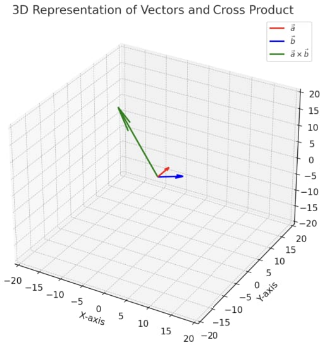
\includegraphics[width=0.8\textwidth]{fig2.7.8}
    \caption{}
    \label{fig:1.2.27.jpg}
\end{figure}

\end{document}